\xchapter{Introduction}{}\section{Context} 
% \label{chapter:introduction}
%

Crisis and emergency are ``sudden and usually unforeseen event that calls for immediate measures to minimise its adverse consequences" \cite{dha1992internationally}. Basically, the term ``crisis communication" is used in two ways: when we refer to communication between organisations involved in managing the crisis and when we refer to necessity of the emergency management to inform and alert the public about the emergency \cite{cdc2014}. The latter definition fits best the scope of our research, being developed considering to minimise the challenges faced by communicators while performing this task. 

Establish an effective communication with the public during a crisis is a key measure for the crisis mitigation. A set of studies \cite{tinker2010}\cite{cdc2014}\cite{glik2007}\cite{seeger2006best} says that is essential maintaining the public informed about the occurrence of an emergency and its consequences. Among the benefits of this action, we can highlight: reduce crisis-related uncertainty; correct misunderstandings, rumours, or unclear facts; and reduce emotional turmoil and anxiety from the public. In addiction, this studies propose good communication principles among which we can highlight some basic principles: be first (for the public the first source is the most reliable); be right (accuracy establishes credibility); be credible (honesty and truthfulness are essential during an crisis); communicate repeatedly (whenever possible, keep the public informed); and communicate by different tools, media and communication channels (never trust on a single method of communication).

%The present solutions for public communication were designed to disseminate a message to many publics. It is an ineffective approach, whereas it the great challenge for the public communication team is creating, quickly, appropriate messages according to the information needs of each public audience during a turbulent moment, like is an emergency.

%Basically, the term ``crisis communication" is used in two ways: when we refer to communication between organisations involved in managing the crisis and when we refer to necessity of the emergency management to inform and alert the public about the emergency \cite{cdc2014}. The latter definition fits best the scope of our research, being developed considering to minimise the challenges faced by communicators while performing this task.

%Several studies have been conducted to propose good communication principles \cite{tinker2010}\cite{cdc2014}\cite{glik2007}, among which we can highlight some basic principles: be first (for the public the first source is the most reliable); be right (accuracy establishes credibility); be credible (honesty and truthfulness are essential during an crisis); communicate repeatedly (whenever possible, keep the public informed); and communicate by different tools, media and communication channels (never trust on a single method of communication).

%Our research, considers all concepts, principles and best practices described previously to propose a  computational model for public communication of emergencies. We mapped the variability in the processor of communications of emergency in order to ensure flexibility of configuration in the different emergency scenarios and/or type of emergencies. Furthermore, we use our variability analysis to design our approach to support customised communication of the emergencies and its consequences targeted to a proper audience. In this approach, we define four variability's behaviour in the content of the sentences according to the emergency state information. Finally, as proof-of-concept we develop a solution for public communication called "RESCUER News". RESCUER News was used during our research by experts of emergency management of two countries (Brazil and Austria), in simulations of emergency occurred in two different scenarios (Industrial Parks and Large Scale Events).

%This research is being developed inside of a larger research project named RESCUER\footnote{Rescuer Project - http://www.rescuer-project.org} -- a joint Brazil-Europe initiative, involving nine research and industry organisations in four countries (Brazil, Austria, Germany and Spain). RESCUER aims at developing an interoperable solution to support command centres in quickly managing emergencies, based on reliable and intelligent analysis of crowdsourcing information mashed up with open data.

\section{Motivation}

In the early hours of December 3, 1984, in the city of Bhopal, India, occurred the biggest chemical disaster for the present day \cite{broughton2005bhopal}. During this incident, 40 tons of toxic products were released into the atmosphere. More than 500 thousand people were exposed to toxic substances, causing 3 thousand direct deaths and 10 thousand due to diseases caused by the inhalation of gases. During the emergency, the managers of the affected factory initially denied the occurrence of emergencies, subsequently claimed to be victims of a terrorist act. Post-tragedy investigations indicated that the real cause was the lack of maintenance and lack of effective security measures as the main causes of the disaster. 

The consequences of these disasters have been amplified due to wrong communication practices. The omission of information from the crisis managers made the medical aid shortfall since the doctors did not know the cause of the intoxication of the hundreds of people who arrived at the hospitals. In addition, measures to protect the population, such as evacuation of communities that would be affected by the toxic cloud in a timely manner, could not be carried out due to a lack of information on the emergencies that were in course.

The disaster that took place in 2016 in the municipality of Mariana in Brazil, caused by the rupture of the retention dam of mining tailings is a recent example of disaster with serious failings in public communication of emergencies. This disaster affected the population of more than 5 districts without any warning from the managers. The tragedy was marked by communication failures to the affected population which caused the death of 19 people dragged through the mud \cite{escobar2015mud}.


During crisis and emergency situations, establish a good communication between the emergency management team and the general public is a key step to minimise the impact on the affected public. However, the process to establish a good communication is not an easy task. Crisis and emergency are complex situations involving stress, panic, fear and uncertainty \cite{reynolds2007crisis} both to the communication team and the people affected directly and indirectly by the consequence of the crisis.

In addiction, the communicators need to ensure that the appropriate messages will be sent to each target audience according to their interests\cite{panamericanhealthorganization2009}. This includes write the messages using appropriate vocabulary, provide you only the most relevant information, ensure the consistency of each message and your trustworthiness. 


Those limitations motivate us to do more detailed research about the process of communication of crisis and emergencies to the public and propose an integrated model in order to help the public communication team write and disseminate appropriated messages according to the interest of each target audience with a reduced effort.

\section{Research Problem}

The current solution for public communication during crisis and emergency situations were designed to disseminating one message to all affected public. In general, those solutions are focused almost totally entirely on the task of disseminating a public communication for several communications channels. The dissemination of messages to the affected public by several communications channel is an important step in the public communications of crisis and emergencies, on the other hand, does not make sense disseminate public communication messages by various communication channels if this message does not meet the information needs of each different target audiences. This is the main problem with this strategy, the dissemination of information that is not in accordance with the information needs of the specific audiences could create an "information overload" in a situation that the public is incapable of juggling multiple facts\cite{cdc2014}. 

Many studies and guides to good practice have been proposed over the last few decades with a view to reducing emergency and service impacts. The problem on the creation and dissemination of public communication during crisis and emergency situations may be explained by the complexity and risk of life's involved on this situations. The need to inform affected people as quickly than possible and ensuring the consistence of the information in a situation that have ``more questions than answers \cite{cdc2014}" is a grant challenger to the emergency communicator.

The solutions proposed for public communication during emergencies focus almost exclusively on the task of disseminating a single message through the most diverse means of communication. The dissemination of information through multiple communication channels is considered a good practice of public communication, but it is not the only challenge for the public communication team. Effective communication with the public during emergencies will, in a simplified way, reliably obtain reliable information, formulate consistent messages and respond to the interests of each public, and finally disseminate them through various communication channels in order to achieve The most amount of stakeholders quickly.

\section{Research Question and Goals}

%The objectives of this research are: 1) to identify public communication challenges coming up in an emergency; 2) to elicit existing users and contextual information needs in an emergency; 3) to define the relevant information adaptation according to different target audiences and phases of an emergency; and 4) to implement this context-aware approach in our RESCUER News systems. The novelty is to support (semi-)automatic customized communication of the incident targeted to different audiences. 

The research question that guides this master thesis is \textbf{“How to reduce the effort of public communication team to transmit relevant and consistent information, according to the interest of each target audience, during the course of an emergency?”}.

The general objective of this dissertation is to present a model for public communication during crisis / emergency situations. To this end, will be made an approach to public communication, elaborated seeking to cover the whole process of communicating of an emergency, that is, obtaining information from reliable sources, making appropriate communications to each target audience and finally, the dissemination of public communications by several communication channels.

To this end, we conceived a model based on the results of our analysis of the variability of the different factors that influence the communication in an emergency; seeking behavioural patterns in the variation of contents of the reports according to the current information of the emergency, the type of incident, the target public, and type of communication (short or extended); variations in the configuration according to the emergency scenario; and in the format of the message according to the different communication channels.

As specific objectives can be cited:

 \begin{itemize}
   \item Make a study of the good practices of emergency communication, especially those that are related to the content that will be transmitted;
   \item Present a new approach to creating documents from dynamic models with behaviours that adapt to the current state of the emergency;
   \item Implementation of a solution for emergency communication based on the proposed model;
   \item Conducting an evaluation with specialists in public communication in real emergency situations to measure quality in use and product in order to validate our proposal.
 \end{itemize}

%\section{Scope Limitation}

\section{Research Benefits}


A contribution from this master thesis is the proposal of a computational model to assist public communicators in the task of creating and disseminating communications during emergency situations. We proposed this model from the survey of the good practices present manuals of good practices in public communication of emergencies and by the practical experience of our partners specialise in the management of the crisis in the industrial park and large scale events.  

Our research also contributes with a study of the variability present in the process of public communication of emergencies, mapping the commonalities in the different aspects relevant to the configuration of an solution for public communication of emergencies or that affect (directly or indirectly) the content of the public communications releases.

An important contribution of our work is our novel approach to generate texts from dynamic models who adapt to the current state of the emergency, in other words, contents can be included or removed automatically according to the type of incident and/or type of Incident that is communicating, for example. In addition, we present four behaviours for varying the content of the sentences of the public communications according to the current status of the emergency.

Finally, another contribution of our work is our emergency communication solution called RESCUER News. We are developing the Rescuer News as a proof-of-concept of our proposed model.

\section{Methodology}

Figure \ref{fig:methodology} presents the methodology, with its phases and activities, considered to achieve the goals of this study.


\begin{figure}[ht!]
\begin{center}
  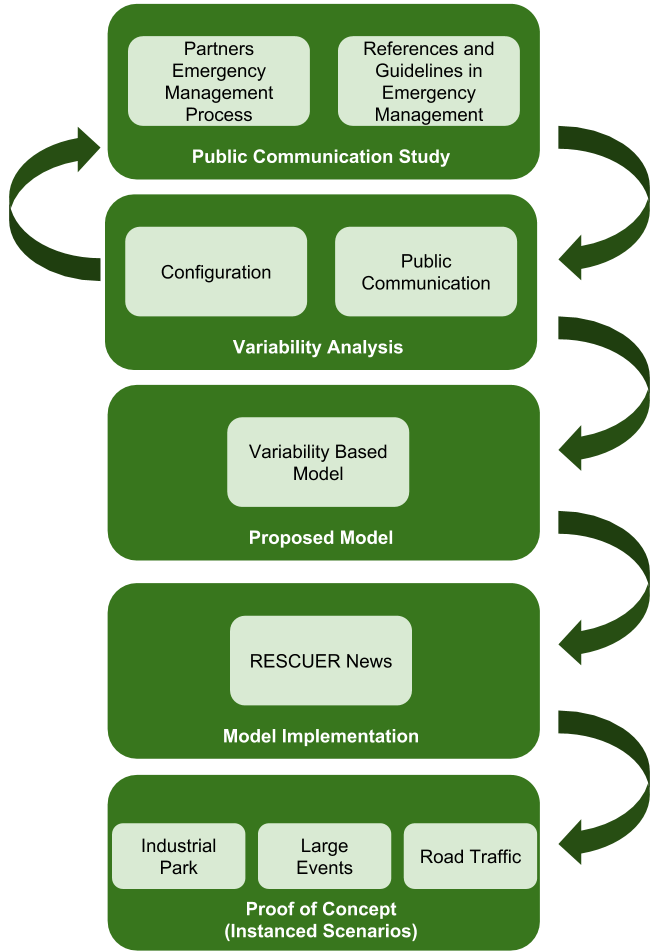
\includegraphics[width=0.50\linewidth, keepaspectratio]{images/Methodology.png}
\caption{Overview of the Research Methodology}
\label{fig:methodology}
\end{center}
\end{figure}


Our research starts with the identification of about how the public communication occurs in real situations. We analysed the processes that our partners applied in these situations and, in parallel, we looked for guides to good practice and manuals for an effective emergency public communication.

After the collection of information, we performed the variability analysis inside of the emergency public communication life cycle.

Next, we developed a conceptual model that would allow configuration for the multiple possible scenarios of an emergency. Based on this model we have developed the RESCUER News, a functional prototype for public communication within ERTK Module of the RESCUER Project.

Finally, as proof of concept we set up our prototype for a series of demonstrations and evaluations within the RESCUER Project.

In the Chapters \ref{chapter:}

\section{Academic Results}

In this section, we present the academic achievements within the scope of this master's thesis.

\subsection{Publications}

During this master's thesis we write the following papers: 

\textbf{Published:}

\begin{itemize}
   \item \emph{Challenges in crowd communication for emergency management}, in Brazilian Congress of Software (CBSOFT), SCrowd 1st WORKSHOP ON CROWDSOURCINGSYSTEMS, 2015 \cite{pereirachallenges};
   
   \item and \emph{Rescuer News: A public communication tool for crisis situations}, Conference on Computer-Supported Cooperative Work and Social Computing (CSCW), Workshop  on  Collaboration  and  Decision  Making  in  Crisis  Situations(CADMICS), 2016 \cite{cscw2016}
  
   \item \emph{On the Design of a Contextual Emergency State Builder with Multiple Data Sources}, First IEEE Summer School on Smart Cities, 2017 \cite{pereiraetall2017}
  
\end{itemize}

\textbf{Submitted:}

\begin{itemize}
   \item \emph{A Variability Based Model to Generate and Disseminate Emergency Public Communications}, in Expert Systems with Applications: An International Journal, 2018 
\end{itemize}

\textbf{Accepted but not published (by authors' choice):}

\begin{itemize}
   \item \emph{Context-Aware Public Communication for Crisis Management}, in The Tenth International Conference on Software Engineering Advances (ICSEA) ,2015 (Short Paper)
\end{itemize}

\textbf{Submitted but not accepted for Publish:}

\begin{itemize}
   \item \emph{Context-Aware Public Communication for Crisis Management}, in ACM Symposium on Applied Computing, 2016 
\end{itemize}


\subsection{Participating in Research Projects}

As mentioned above, this research was developed inside of the Rescuer Project, more specifically, as part of the ERTK component. 

Among the activities developed in the project we can highlight: a study on public communication of emergencies including the organisation of 4 workshops with specialist in crisis communication; the publication of two articles in workshops focused on crisis and emergencies; organisation of simulation to evaluate the prototypes developed in the project; and the development of a solution for communication with the public during crisis and emergencies called ``Rescue NEWS". 


\subsection{Research Exchange}

Research Interchange was conducted during the 1 year period (October 2015 to November 2016) as a invited researcher at the Fraunhofer Institute for Experimental Software Engineering (IESE)\footnote{https://www.iese.fraunhofer.de/en.html}, in the city of Kaiserslautern, Germany. The IESE is one of the most widely recognized software engineering institutions world-wide and takes a lead in Europe. Among your competences, we can highlight: Requirements Engineering,  Software Architecture, Safety Engineering and User Experience.

During the period in the institute, the student worked on tasks related to his master's research and on tasks related to performing demonstrations and evaluations of the components of the RESCUER Project.

\section{Document structure}

The remainder of this text is structured as follows: Chapter \ref{cap:2} presents the main concept of emergency public communication, the related work in document variability and an analysis of the present solution for public communication

Chapter \ref{cap:3} we present our mapping of variability in the process of public communication of emergencies, the conceptual model proposed in this research, the academic results and our activity schedule from the rest of this master thesis.